
\documentclass[a4paper,11pt]{article}
\usepackage{geometry}
\geometry{margin=2cm}
\usepackage{booktabs}
\usepackage{graphicx}
\usepackage{amsmath}
\usepackage{siunitx}
\usepackage{caption}
\usepackage{times}
\usepackage[utf8]{inputenc}
\usepackage{tocloft}
\usepackage{pdflscape} % Mengganti rotating dengan pdflscape untuk landscape

\title{Spectral Simulation Report}
\author{Automated Analysis}
\date{\today}

\begin{document}

\maketitle
\tableofcontents
\clearpage

\section{Introduction}
This report presents the results of spectral simulations derived from HDF5 dataset analysis. Each sample includes a spectral plot displayed in a full horizontal page and a detailed table summarizing the initial composition, actual positions, total pixels, and signal-to-noise ratio (SNR), along with simulation parameters such as temperature and electron density.


\section{Sample: 12098}
\subsection{Simulation Parameters}
\begin{table}[h!]
    \centering
    \begin{tabular}{ll}
        \toprule
        \textbf{Parameter} & \textbf{Value} \\
        \midrule
        Temperature ($T$) & 10657 \,\si{K} \\
        Electron Density ($n_e$) & 4.53e+15 \,\si{cm^-3} \\
        Total Pixels & 4096 \\
        Signal-to-Noise Ratio (SNR) & 47.04 \\
        \bottomrule
    \end{tabular}
    \caption{Simulation parameters and additional metrics for sample 12098.}
    \label{tab:params_12098}
\end{table}

\subsection{Composition Analysis}
\begin{table}[h!]
    \centering
    \begin{tabular}{lcc}
        \toprule
        \textbf{Element} & \textbf{Initial Composition (\%)} & \textbf{Actual Positions} \\
        \midrule
        Al & 17.44 & 462.0 \\
        Ar & 0.00 & 0.0 \\
        C & 0.00 & 0.0 \\
        Ca & 17.25 & 150.0 \\
        Cl & 15.49 & 35.0 \\
        Co & 0.00 & 0.0 \\
        Cr & 4.88 & 397.0 \\
        Fe & 0.00 & 0.0 \\
        Mg & 4.21 & 352.0 \\
        Mn & 16.98 & 706.0 \\
        N & 0.00 & 0.0 \\
        Na & 2.39 & 322.0 \\
        Ni & 6.40 & 478.0 \\
        O & 0.00 & 0.0 \\
        S & 11.11 & 228.0 \\
        Si & 3.85 & 221.0 \\
        Ti & 0.00 & 0.0 \\
        background & N/A & 1847.0 \\

        \midrule
        \textbf{Total Positions} & & 5198.0 \\
        \bottomrule
    \end{tabular}
    \caption{Composition analysis for sample 12098.}
    \label{tab:comp_12098}
\end{table}

\subsection{Spectral Plot}
\begin{figure}[p]
    \begin{landscape}
        \centering
        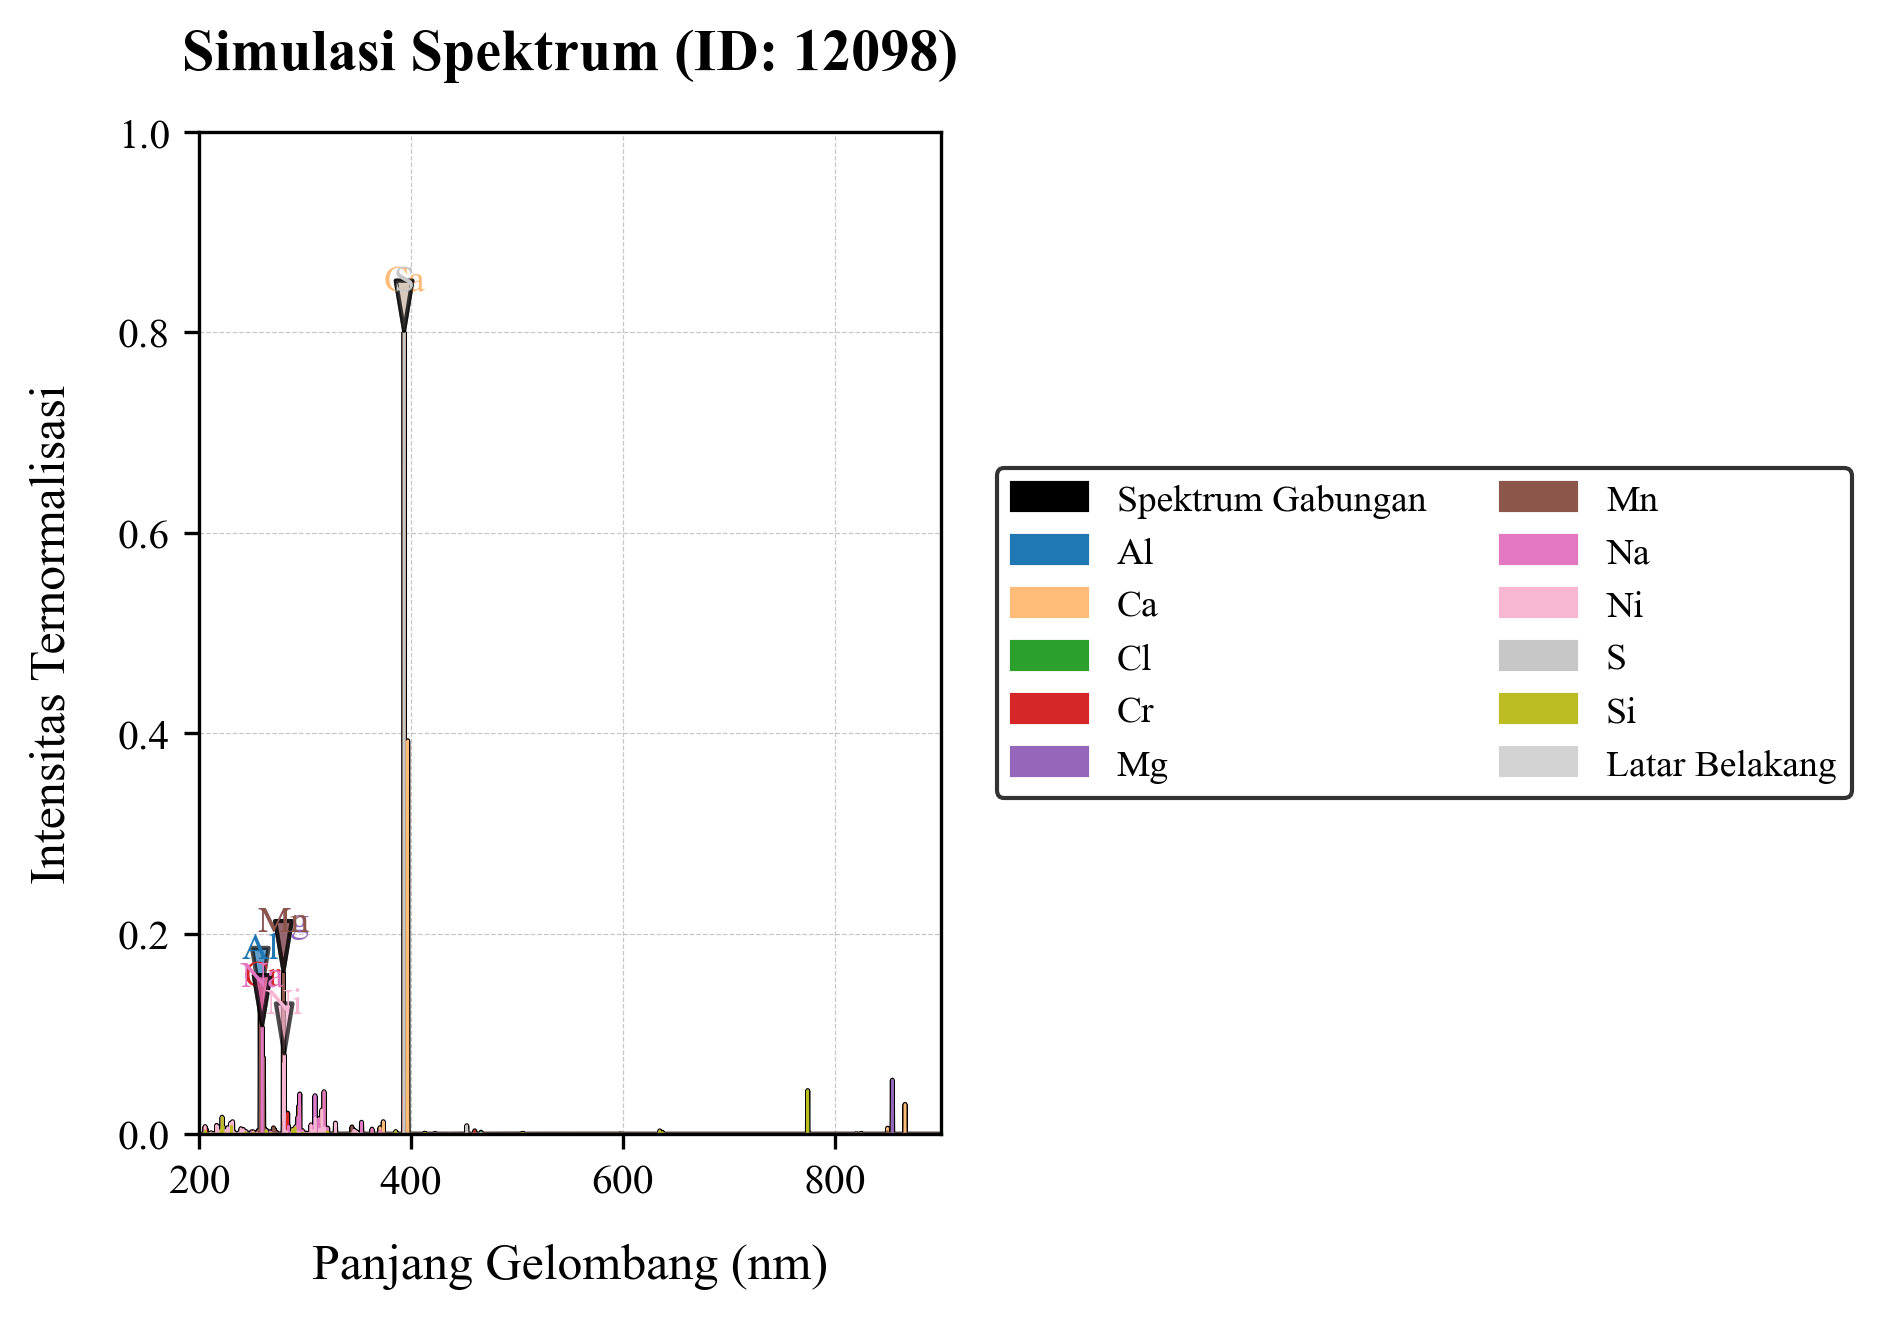
\includegraphics[width=1.2\textwidth, angle=90]{spectrum_12098.png}
        \caption{Spectral simulation plot for sample 12098 in full horizontal layout.}
        \label{fig:spectrum_12098}
    \end{landscape}
\end{figure}

\clearpage

\section{Sample: 15240}
\subsection{Simulation Parameters}
\begin{table}[h!]
    \centering
    \begin{tabular}{ll}
        \toprule
        \textbf{Parameter} & \textbf{Value} \\
        \midrule
        Temperature ($T$) & 7929 \,\si{K} \\
        Electron Density ($n_e$) & 4.98e+15 \,\si{cm^-3} \\
        Total Pixels & 4096 \\
        Signal-to-Noise Ratio (SNR) & 35.07 \\
        \bottomrule
    \end{tabular}
    \caption{Simulation parameters and additional metrics for sample 15240.}
    \label{tab:params_15240}
\end{table}

\subsection{Composition Analysis}
\begin{table}[h!]
    \centering
    \begin{tabular}{lcc}
        \toprule
        \textbf{Element} & \textbf{Initial Composition (\%)} & \textbf{Actual Positions} \\
        \midrule
        Al & 4.11 & 287.0 \\
        Ar & 10.89 & 725.0 \\
        C & 5.07 & 224.0 \\
        Ca & 11.61 & 150.0 \\
        Cl & 3.67 & 12.0 \\
        Co & 0.00 & 0.0 \\
        Cr & 10.33 & 397.0 \\
        Fe & 0.00 & 0.0 \\
        Mg & 4.64 & 326.0 \\
        Mn & 2.97 & 706.0 \\
        N & 2.81 & 396.0 \\
        Na & 9.54 & 325.0 \\
        Ni & 4.60 & 478.0 \\
        O & 9.70 & 117.0 \\
        S & 8.18 & 77.0 \\
        Si & 5.14 & 218.0 \\
        Ti & 6.75 & 1184.0 \\
        background & N/A & 1144.0 \\

        \midrule
        \textbf{Total Positions} & & 6766.0 \\
        \bottomrule
    \end{tabular}
    \caption{Composition analysis for sample 15240.}
    \label{tab:comp_15240}
\end{table}

\subsection{Spectral Plot}
\begin{figure}[p]
    \begin{landscape}
        \centering
        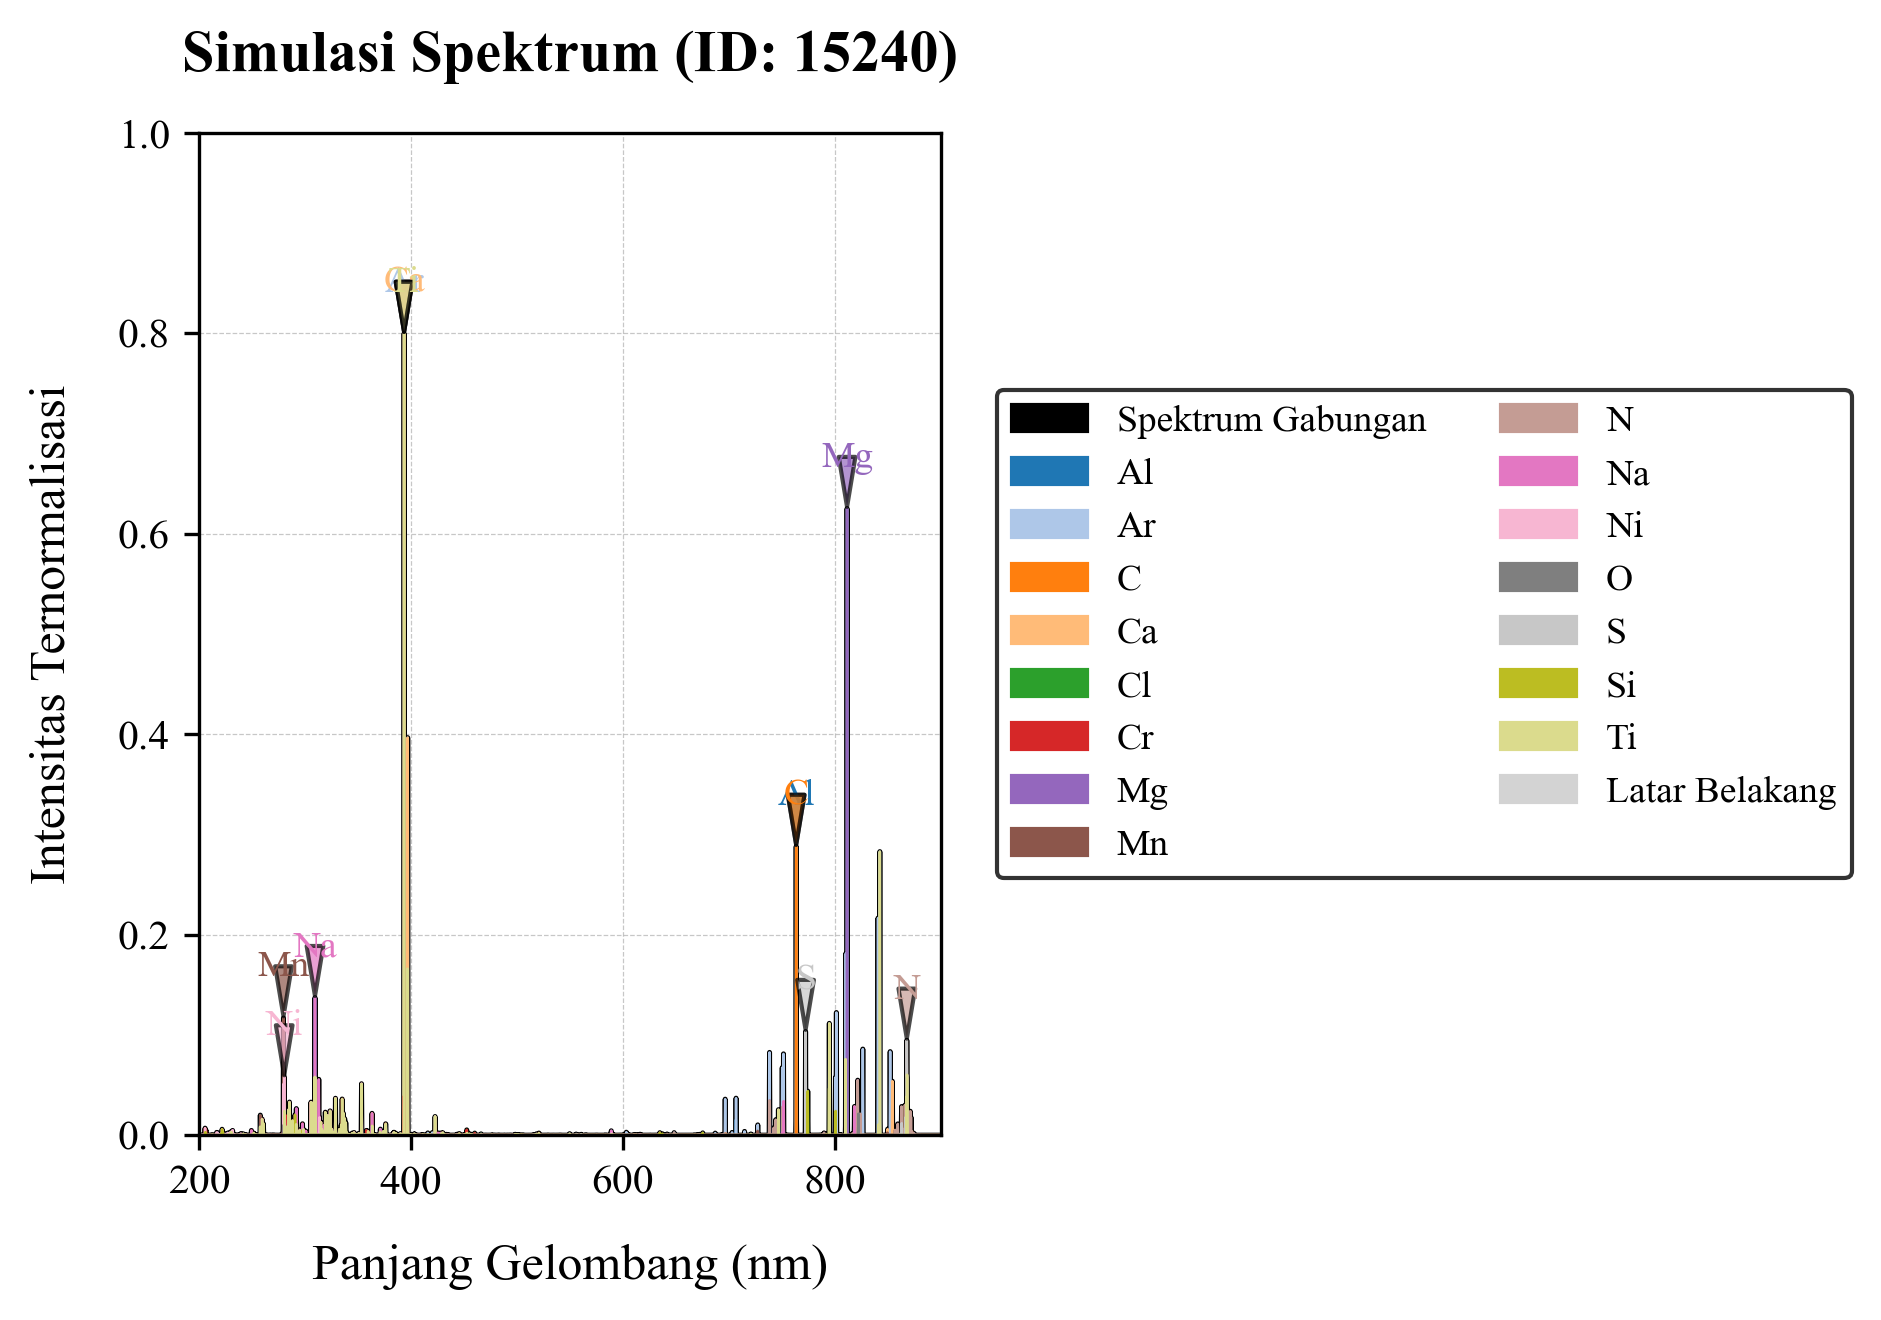
\includegraphics[width=1.2\textwidth, angle=90]{spectrum_15240.png}
        \caption{Spectral simulation plot for sample 15240 in full horizontal layout.}
        \label{fig:spectrum_15240}
    \end{landscape}
\end{figure}

\clearpage

\section{Sample: 14064}
\subsection{Simulation Parameters}
\begin{table}[h!]
    \centering
    \begin{tabular}{ll}
        \toprule
        \textbf{Parameter} & \textbf{Value} \\
        \midrule
        Temperature ($T$) & 6111 \,\si{K} \\
        Electron Density ($n_e$) & 1.12e+15 \,\si{cm^-3} \\
        Total Pixels & 4096 \\
        Signal-to-Noise Ratio (SNR) & 47.65 \\
        \bottomrule
    \end{tabular}
    \caption{Simulation parameters and additional metrics for sample 14064.}
    \label{tab:params_14064}
\end{table}

\subsection{Composition Analysis}
\begin{table}[h!]
    \centering
    \begin{tabular}{lcc}
        \toprule
        \textbf{Element} & \textbf{Initial Composition (\%)} & \textbf{Actual Positions} \\
        \midrule
        Al & 12.98 & 157.0 \\
        Ar & 0.00 & 0.0 \\
        C & 0.00 & 0.0 \\
        Ca & 22.75 & 150.0 \\
        Cl & 2.85 & 12.0 \\
        Co & 0.00 & 0.0 \\
        Cr & 3.80 & 397.0 \\
        Fe & 0.00 & 0.0 \\
        Mg & 13.14 & 183.0 \\
        Mn & 11.93 & 681.0 \\
        N & 0.00 & 0.0 \\
        Na & 10.30 & 325.0 \\
        Ni & 3.77 & 478.0 \\
        O & 17.07 & 27.0 \\
        S & 0.48 & 25.0 \\
        Si & 0.93 & 177.0 \\
        Ti & 0.00 & 0.0 \\
        background & N/A & 2278.0 \\

        \midrule
        \textbf{Total Positions} & & 4890.0 \\
        \bottomrule
    \end{tabular}
    \caption{Composition analysis for sample 14064.}
    \label{tab:comp_14064}
\end{table}

\subsection{Spectral Plot}
\begin{figure}[p]
    \begin{landscape}
        \centering
        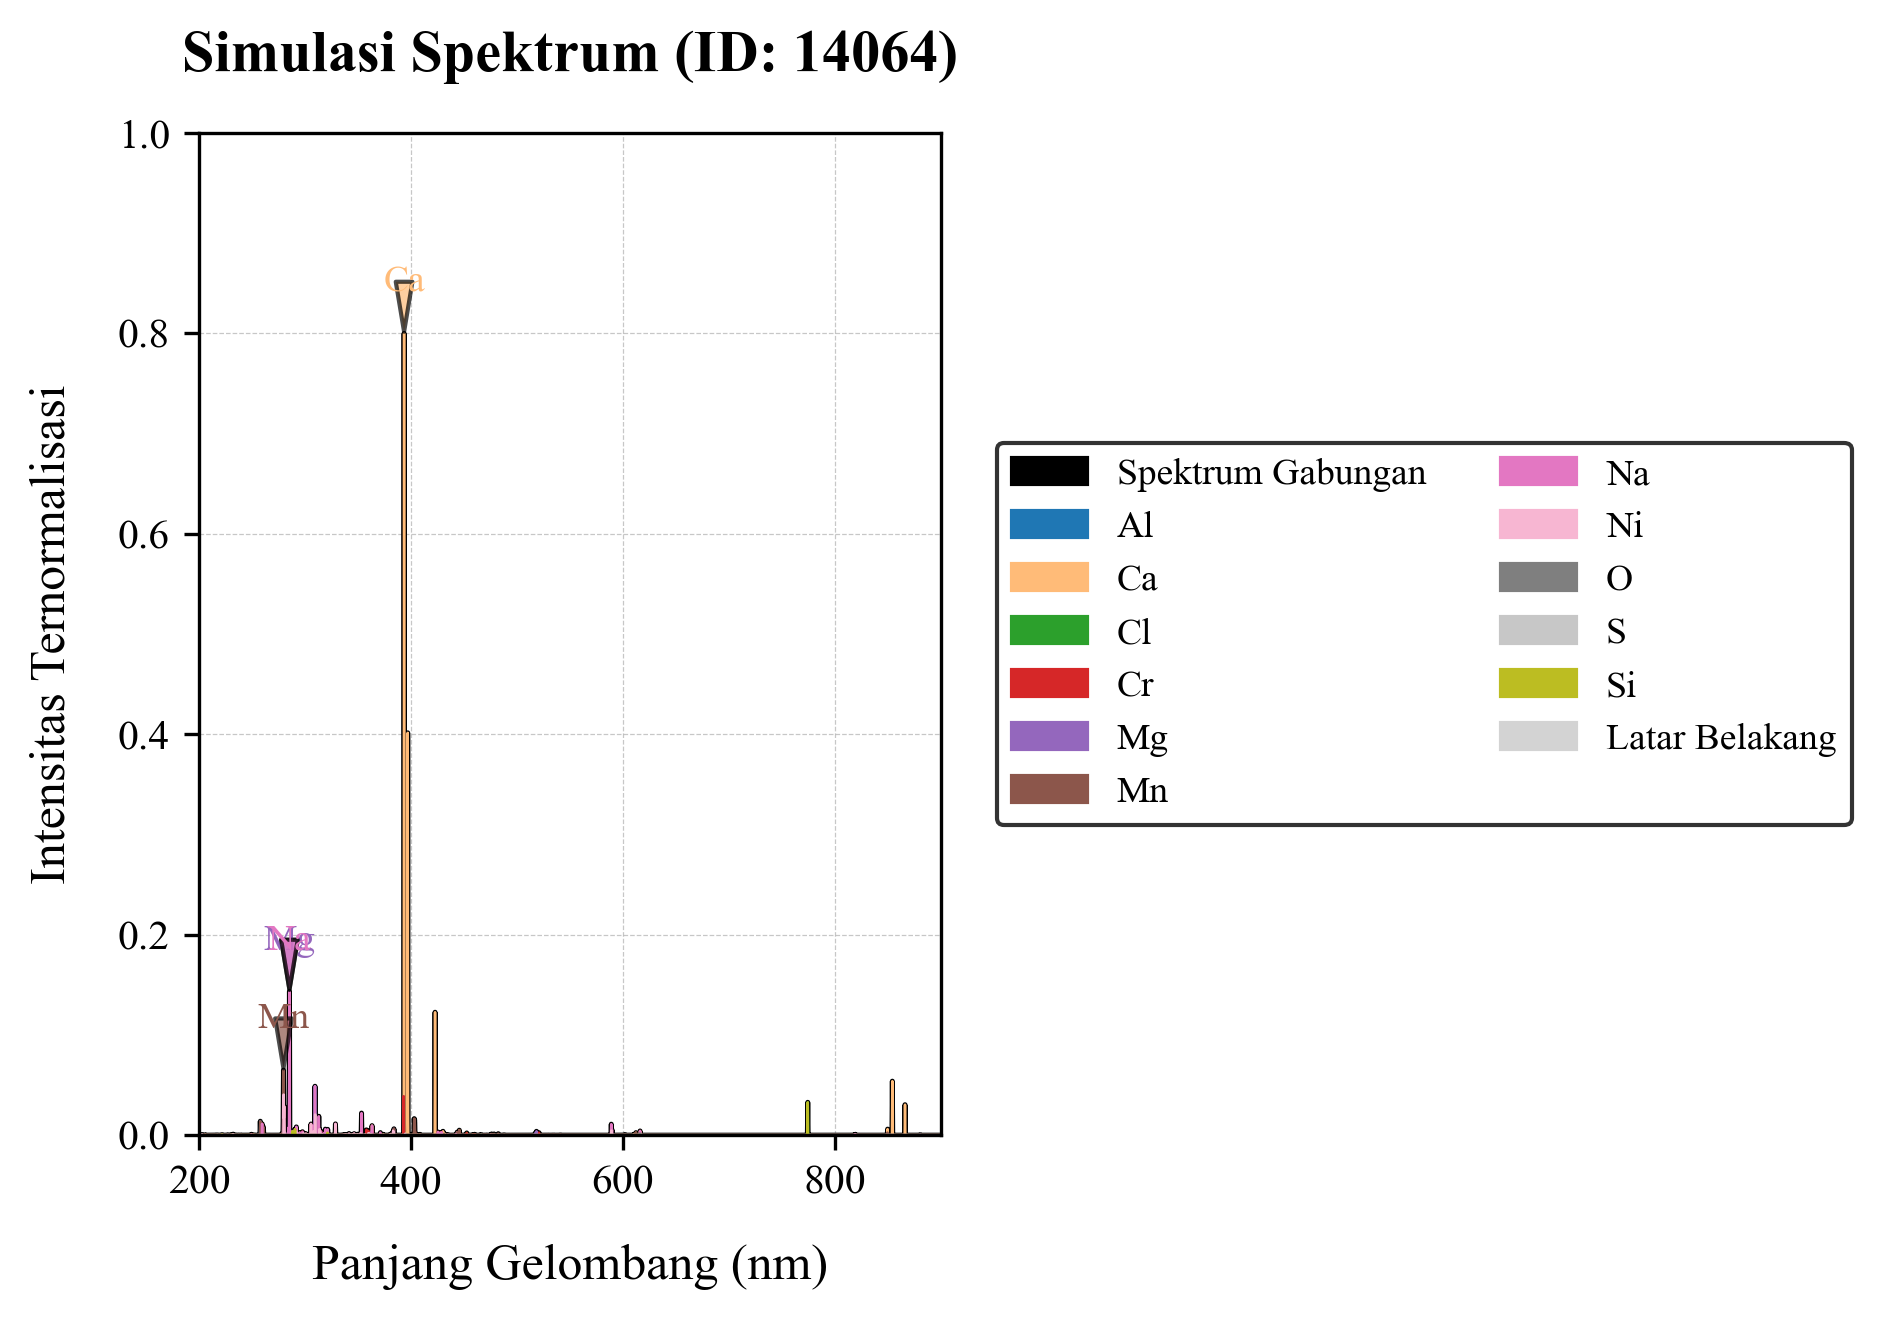
\includegraphics[width=1.2\textwidth, angle=90]{spectrum_14064.png}
        \caption{Spectral simulation plot for sample 14064 in full horizontal layout.}
        \label{fig:spectrum_14064}
    \end{landscape}
\end{figure}

\clearpage

\section{Sample: 8780}
\subsection{Simulation Parameters}
\begin{table}[h!]
    \centering
    \begin{tabular}{ll}
        \toprule
        \textbf{Parameter} & \textbf{Value} \\
        \midrule
        Temperature ($T$) & 9040 \,\si{K} \\
        Electron Density ($n_e$) & 1.10e+14 \,\si{cm^-3} \\
        Total Pixels & 4096 \\
        Signal-to-Noise Ratio (SNR) & 26.98 \\
        \bottomrule
    \end{tabular}
    \caption{Simulation parameters and additional metrics for sample 8780.}
    \label{tab:params_8780}
\end{table}

\subsection{Composition Analysis}
\begin{table}[h!]
    \centering
    \begin{tabular}{lcc}
        \toprule
        \textbf{Element} & \textbf{Initial Composition (\%)} & \textbf{Actual Positions} \\
        \midrule
        Al & 0.00 & 0.0 \\
        Ar & 8.49 & 727.0 \\
        C & 9.50 & 255.0 \\
        Ca & 5.25 & 150.0 \\
        Cl & 7.49 & 35.0 \\
        Co & 9.50 & 1404.0 \\
        Cr & 6.45 & 397.0 \\
        Fe & 9.51 & 2740.0 \\
        Mg & 6.46 & 341.0 \\
        Mn & 5.52 & 706.0 \\
        N & 8.48 & 401.0 \\
        Na & 8.67 & 321.0 \\
        Ni & 3.51 & 473.0 \\
        O & 1.13 & 107.0 \\
        S & 2.41 & 205.0 \\
        Si & 7.65 & 223.0 \\
        Ti & 0.00 & 0.0 \\
        background & N/A & 511.0 \\

        \midrule
        \textbf{Total Positions} & & 8996.0 \\
        \bottomrule
    \end{tabular}
    \caption{Composition analysis for sample 8780.}
    \label{tab:comp_8780}
\end{table}

\subsection{Spectral Plot}
\begin{figure}[p]
    \begin{landscape}
        \centering
        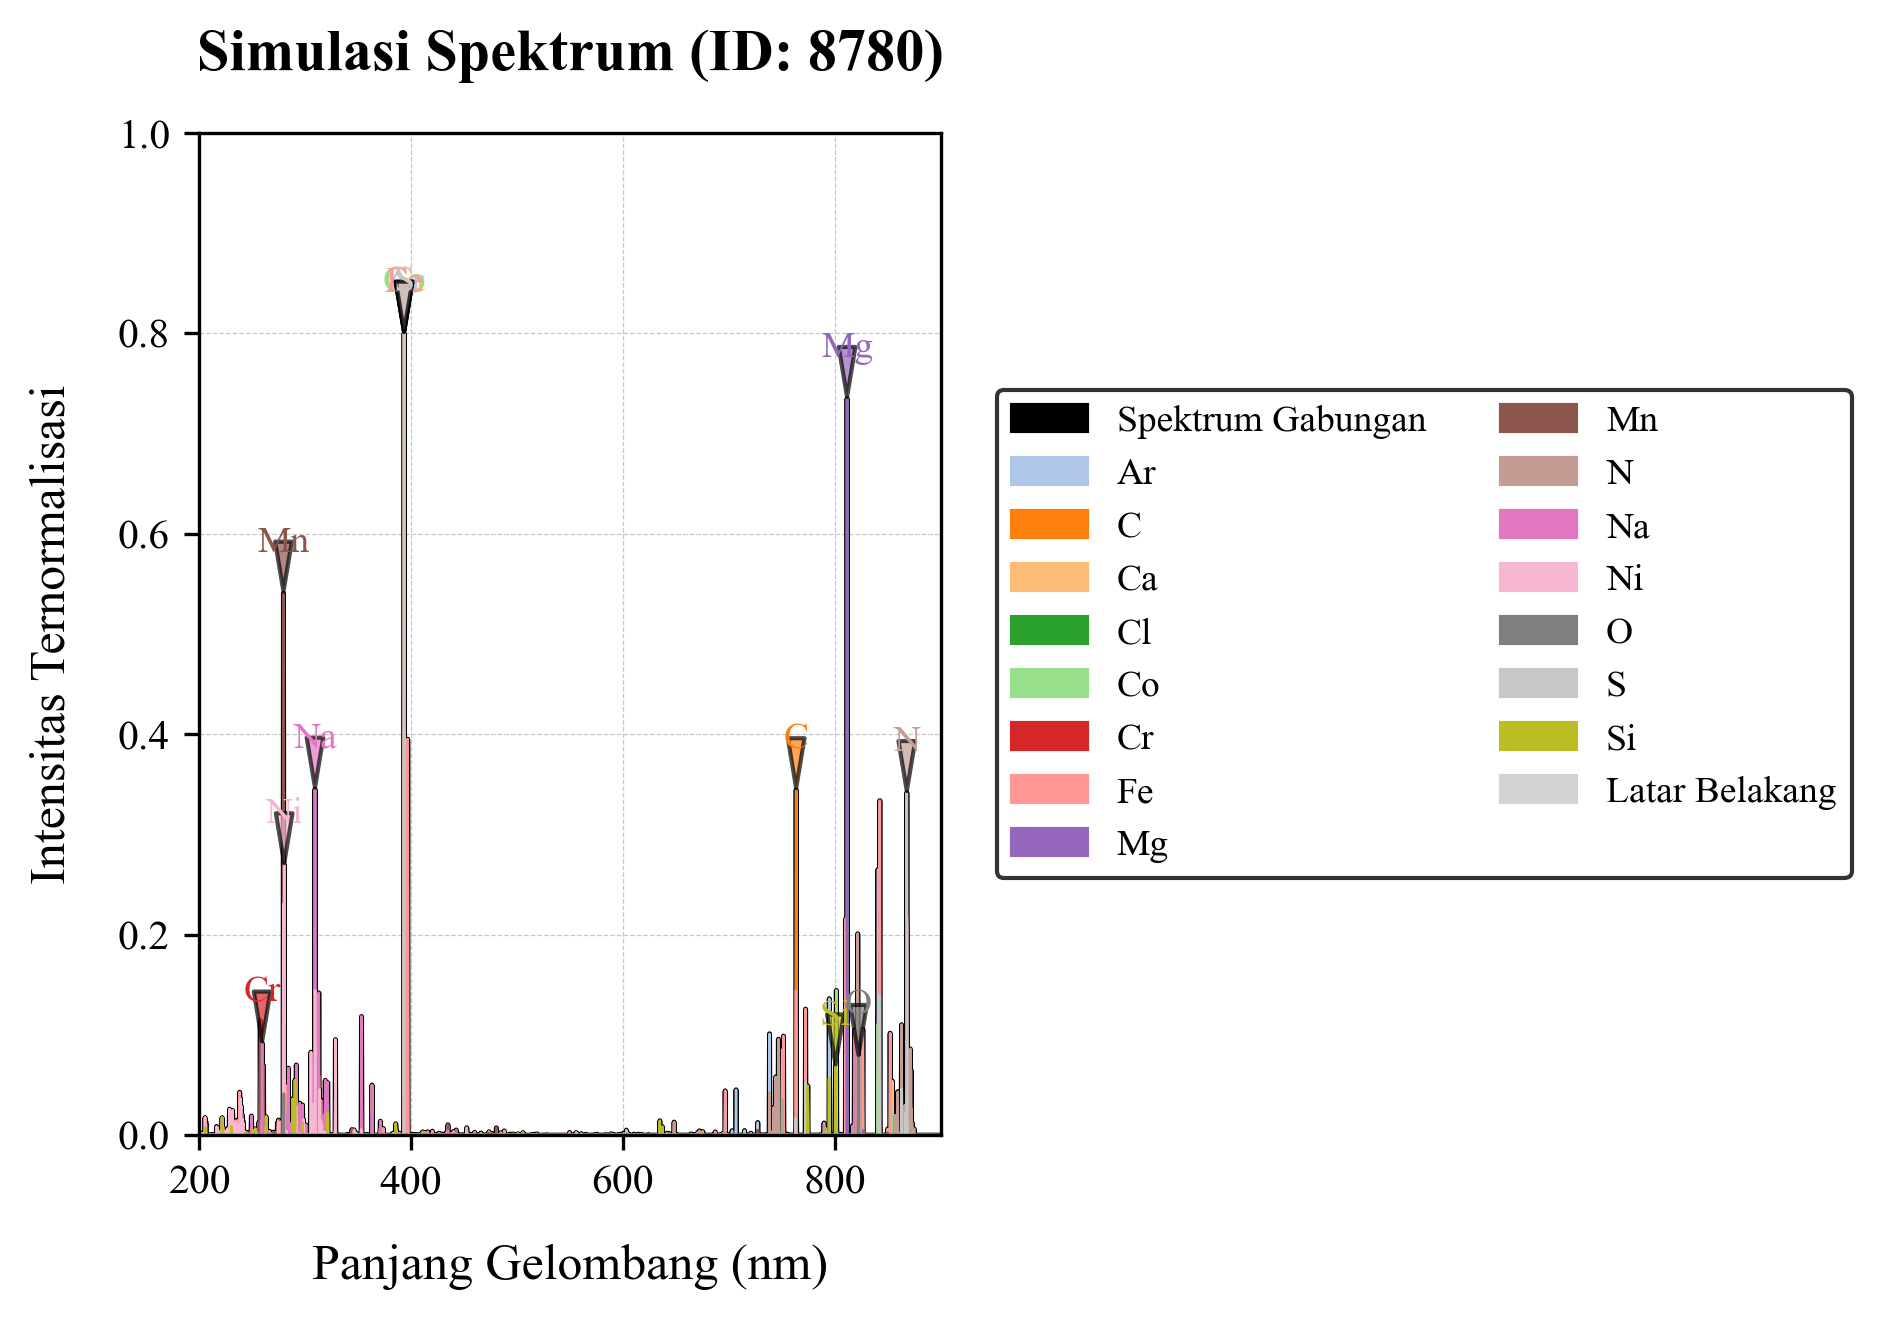
\includegraphics[width=1.2\textwidth, angle=90]{spectrum_8780.png}
        \caption{Spectral simulation plot for sample 8780 in full horizontal layout.}
        \label{fig:spectrum_8780}
    \end{landscape}
\end{figure}

\clearpage

\section{Sample: 10667}
\subsection{Simulation Parameters}
\begin{table}[h!]
    \centering
    \begin{tabular}{ll}
        \toprule
        \textbf{Parameter} & \textbf{Value} \\
        \midrule
        Temperature ($T$) & 7727 \,\si{K} \\
        Electron Density ($n_e$) & 1.79e+15 \,\si{cm^-3} \\
        Total Pixels & 4096 \\
        Signal-to-Noise Ratio (SNR) & 40.14 \\
        \bottomrule
    \end{tabular}
    \caption{Simulation parameters and additional metrics for sample 10667.}
    \label{tab:params_10667}
\end{table}

\subsection{Composition Analysis}
\begin{table}[h!]
    \centering
    \begin{tabular}{lcc}
        \toprule
        \textbf{Element} & \textbf{Initial Composition (\%)} & \textbf{Actual Positions} \\
        \midrule
        Al & 6.22 & 279.0 \\
        Ar & 0.00 & 0.0 \\
        C & 0.00 & 0.0 \\
        Ca & 8.18 & 150.0 \\
        Cl & 5.11 & 12.0 \\
        Co & 10.87 & 1404.0 \\
        Cr & 3.96 & 397.0 \\
        Fe & 2.63 & 2704.0 \\
        Mg & 7.52 & 326.0 \\
        Mn & 8.90 & 706.0 \\
        N & 6.53 & 396.0 \\
        Na & 4.75 & 322.0 \\
        Ni & 8.70 & 478.0 \\
        O & 9.24 & 101.0 \\
        S & 5.65 & 61.0 \\
        Si & 5.76 & 220.0 \\
        Ti & 5.97 & 1184.0 \\
        background & N/A & 590.0 \\

        \midrule
        \textbf{Total Positions} & & 9330.0 \\
        \bottomrule
    \end{tabular}
    \caption{Composition analysis for sample 10667.}
    \label{tab:comp_10667}
\end{table}

\subsection{Spectral Plot}
\begin{figure}[p]
    \begin{landscape}
        \centering
        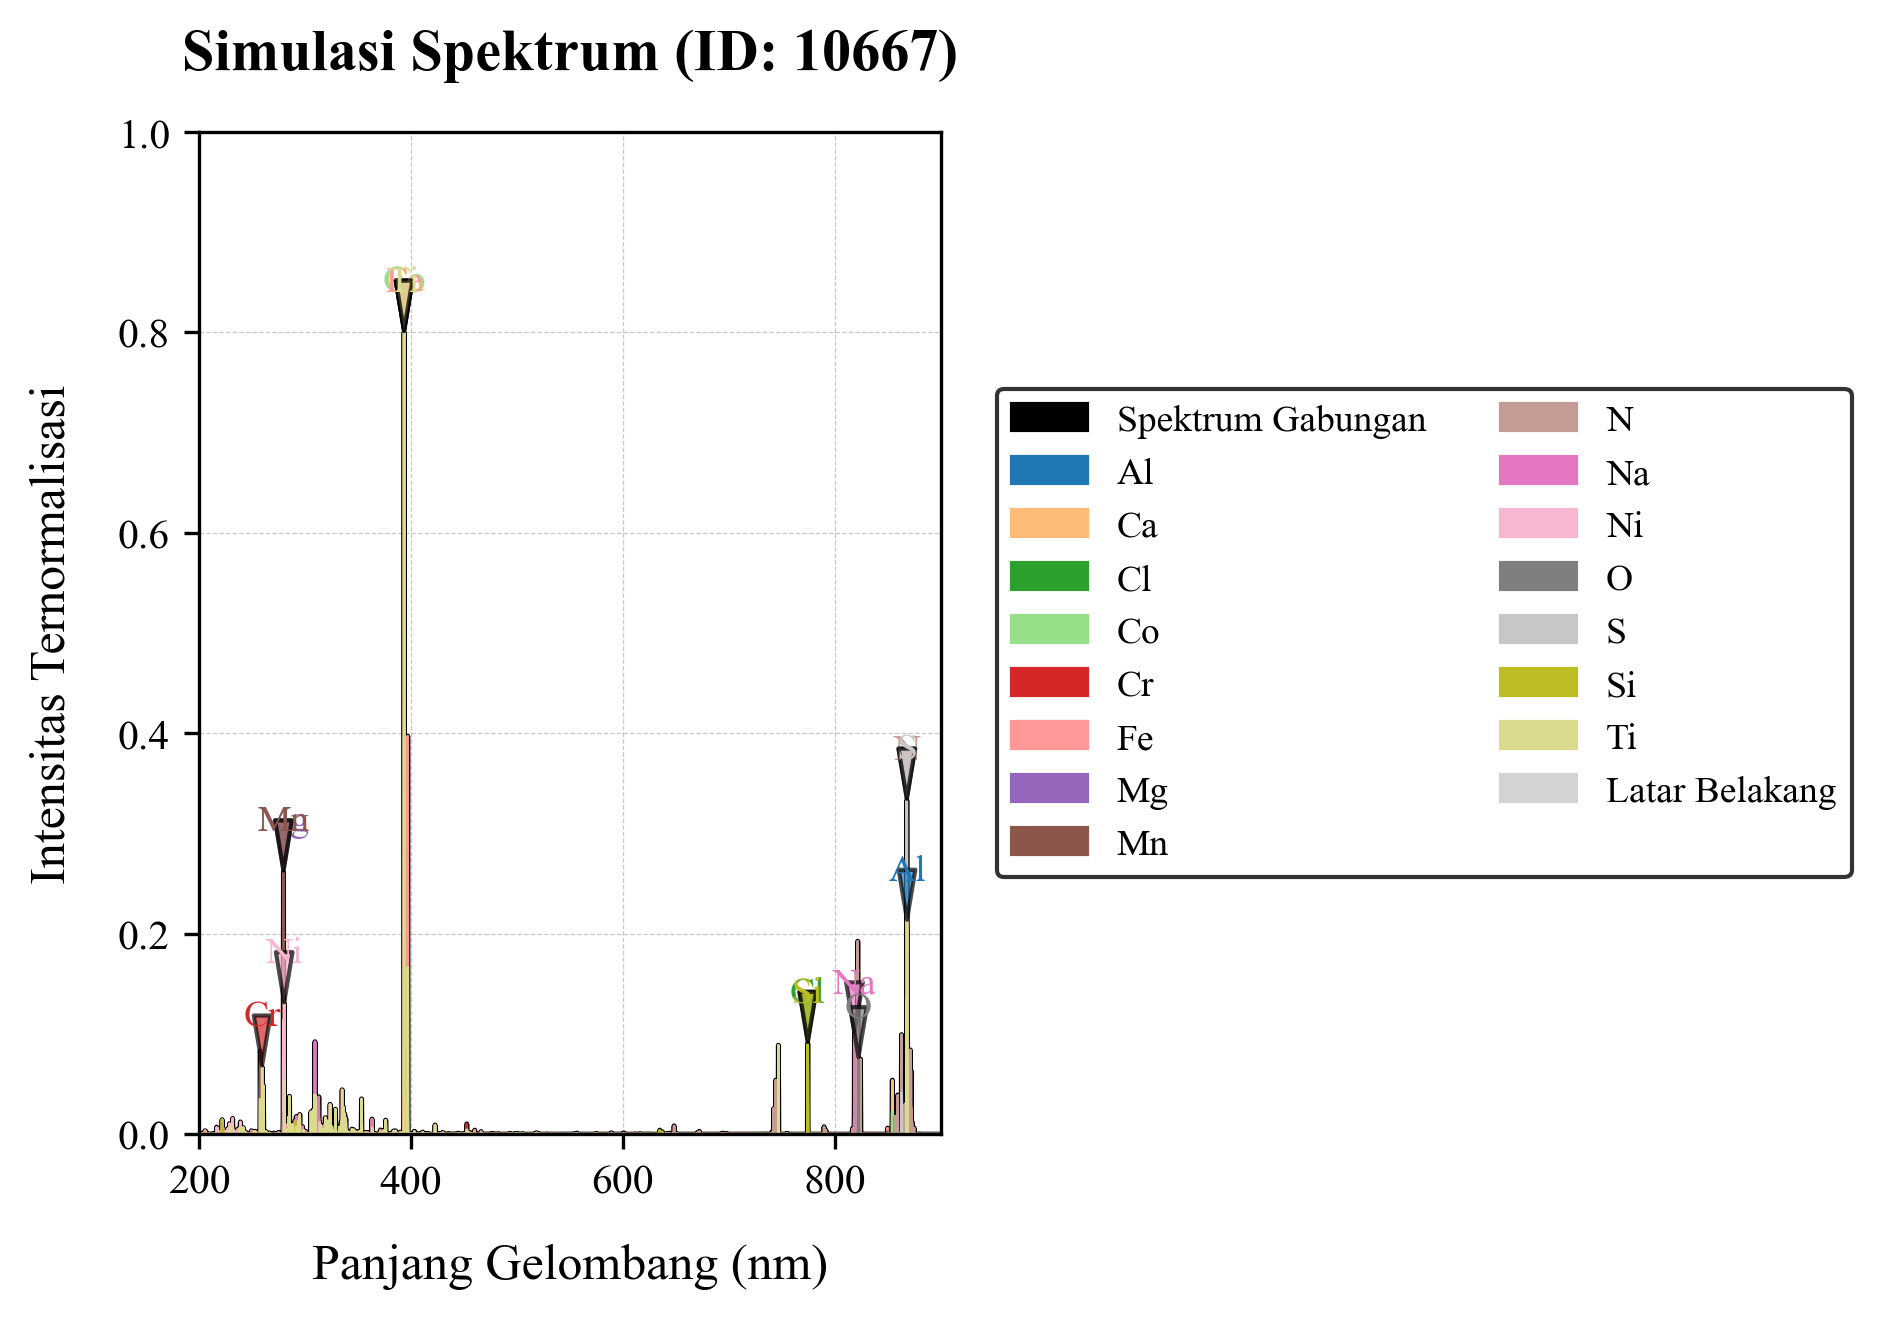
\includegraphics[width=1.2\textwidth, angle=90]{spectrum_10667.png}
        \caption{Spectral simulation plot for sample 10667 in full horizontal layout.}
        \label{fig:spectrum_10667}
    \end{landscape}
\end{figure}

\clearpage

\end{document}
